\documentclass[a4paper]{article}
\renewcommand{\baselinestretch}{1.5}
\usepackage[margin=2cm]{geometry}
\usepackage{float}
\usepackage{enumerate}

\usepackage{graphicx}
\usepackage{color}
\usepackage{mhchem}
\usepackage{physics}
\usepackage[font=small, labelfont=bf]{caption}
\usepackage{subcaption}
\usepackage{wrapfig}
\usepackage{framed}
\usepackage{hyperref} 
\usepackage[numbers]{natbib}


\setlength{\droptitle}{-4cm}
\setlength{\parindent}{0pt}

\newcommand*\chem[1]{\ensuremath{\mathrm{#1}}}
\def\rf{{\ensuremath{r_{\mathrm{F}}}}}
\def\rref{{\ensuremath{r_{\mathrm{ref}}}}}
\def\rdiff{{\ensuremath{r_{\mathrm{diff}}}}}
\def\tdiff{{\ensuremath{\theta_{\mathrm{diff}}}}}
\def\tscatt{{\ensuremath{\theta_{\mathrm{scatt}}}}}
\def\halpha{$\mathrm{H\alpha}$\;}
\def\sm{\texttt{SM2017}}

\begin{document}
\title{Dissertation layout}
\tableofcontents{}
\newpage
\section{Literature Review}
%\include{Hon_LR_Final.tex}
\section{Calculations / Program}
In the previous section we summarised the background of the project and some of the key methods that would be used in our program. In this section we will go through the programs and calculations used to simulate variability. To do this we must first obtain the scattering measure along a line of sight using Hydrogen Alpha, assumptions about the turbulent nature of the gas and a model of strong refractive scattering (RISS). The program that does these calculations is \texttt{SM2017}.

\subsection{SM2017}\label{sec:SM2017}
The simulation runs off the basis of \texttt{SM2017} model, written by Dr. Paul Hancock. More information is detailed in \texttt{SM2017} PAPER\citet{H18}. Here we will concisely lay out how the \texttt{SM2017} program works and what modifications were made to it. In summary \texttt{SM2017} works by taking in a position(s) and returning a Hydrogen Alpha Intensity value at this specified position. We can then intrinsically link Hydrogen Alpha to the Scattering Measure through some assumptions using the following Equation \ref{eq:SMfull}, as described in \citet{Haffner}.
\begin{equation}
\mathrm{SM} = \left(\frac{\mathrm{I_{H_\alpha}}}{198R}\right)T_4^{0.9}\frac{\varepsilon^{2}}{(1+\varepsilon^2)}\ell_0^{-2/3}\, (\mathrm{kpc.m}^{-20/3})
\label{eq:SMfull}
\end{equation}
Where $I_{H_\alpha}$ is measured in Rayleighs, $T_4$ is the gas temperature in units of $10^4$\,K, $\varepsilon$ is the fractional variance of $n_e$ inside clouds , and $\ell_0$ is the outer scale of turbulence in units of pc.
The \sm model uses the following values $\varepsilon = 1$,  $T_4=0.8$ \citep{Haffner}, and $\ell_0 = 10^{18}m = 32pc$ \citep{Armstrong}.
Using these values we can get a more simplified form of the linear relation between the scattering measure and the \halpha{} intensity:
\begin{equation}
\mathrm{SM} = 1.26\times 10^{16} I_{H_\alpha}\, (\mathrm{m}^{-17/3})
\label{eq:SMshort}
\end{equation}

\texttt{SM2017} then derives the scattering measure $\mathrm{r_{diff}}$ through Kolomogorov modelling of the turbulence and the assumption that the scattering disk is within our galaxay, as described in \citet{JP}.
\begin{equation}
\rdiff = 3.7\times 10^9 \left(\frac{\lambda}{1m}\right)^{-6/5} \left(\frac{SM}{10^{12} m^{-17/3}}\right)^{-3/5}\, (\mathrm{m})
\end{equation}
\texttt{SM2017} then uses the two scattering measures ($\mathrm{r_{diff}}$ and $\mathrm{r_{F}}$) to calculate the refractive length scale which in turn is used to calculate the angular size of the scattering disk. 
\begin{equation}
    \rref = \rf^2 / \rdiff
\end{equation}
\begin{equation}
    \tscatt = \rref / D 
\end{equation}
Recalling from Equation \ref{eq:rf} that the Fresnel scale can be wrriten as:
\[\mathrm{
r_F=\sqrt{\dfrac{\lambda D}{2 \pi}}
}\]
Where D is the distance to the scattering screen and $\lambda$ is the wavelength of the observation. \tetttt{SM2017} makes the assumption that the scattering screen is 1 kpc away which is a common distance used for scaterring screens. These quantities are then used to calculate the modulation index.
\begin{equation}\label{eq:mp}
   m_p=\bigg(\dfrac{r_{\mathrm{diff}}}{r_{\mathrm{F}}}\bigg)^{1/3}
\end{equation}
\begin{equation}\label{eq:me}
   m_e=\bigg(\dfrac{r_{\mathrm{diff}}}{r_{\mathrm{F}}}\bigg)^{1/3}\bigg(\dfrac{\theta_{\mathrm{scatt}}}{\theta_\mathrm{S}}\bigg)^{7/6}
\end{equation}
The \texttt{SM2017} model also calculates other parameters: Transition Frequency, RMS variations and the refractive timescale. The refractive time scale is important as it is used in the Simulation to scale the modulation index, however the others we not used.
\ref{eq:tref}.
\begin{equation}\label{eq:tref}
    t_\mathrm{ref} = \rref / v
\end{equation}
Originally the \texttt{SM2017} basis just did point source modulation calculations (Equation \ref{eq:mp}) but it has now been modified so that it can now calculate for extended sources if need be. Originally this was not done as it required an input of source size from the user. We also added error calculations to all the outputted parameters using the Hydrogen Alpha Error Map. A summation of the \texttt{SM2017} program in visual form can be seen in Figure \ref{fig:SM}.
\begin{figure}[H]
    \centering
    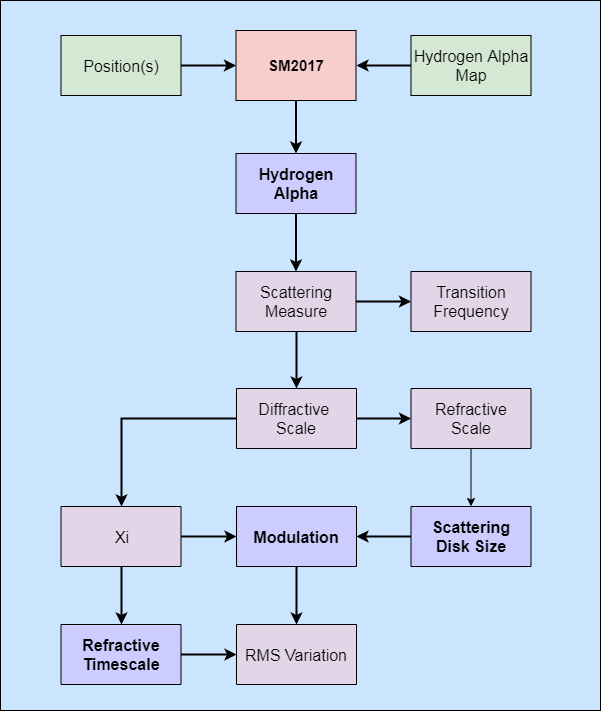
\includegraphics[width=0.6\textwidth]{SM2017.png}
    \caption{\texttt{SM2017} program flowchart. Where Green are the input data, Red is the actual program, Pink are outputs and Purple with bold text are outputs that are used in the Simulation Program.}
    \label{fig:SM}
\end{figure}

Now that we have a program that calculates the variability (modulation index) for given line of sights, we now want to be able to apply this to a given survey region and to populate this region with sources. This is done using the \texttt{Simulation} program.
\subsection{Simulation}
The idea behind the simulation is to take a region given as well as some other parameters and to generate information from this region to feed into the \texttt{SM2017} base. The first step is to generate the correct number of sources at the correct flux level, this is called the source counts. Using a source count model we can generate the number of sources at a certain flux to populate the region, then calculate variability using this information. We can write the source count function in its differential form in Equation \ref{eq:dnds}.
\begin{equation}\label{eq:dnds}
    \dfrac{dN}{dS}= \alpha S^{-\beta} \; \mathrm{(Jy^{-1} \; sr^{-1})}
\end{equation}
Where alpha is a scale factor to account for missing source counts which can be changed in the simulation but is set to a default of 3300 as inferred from Table 5 in \citet{Intema}. Beta is the power law slope and is equal to 1.6 for sources below 1 Jy. If we integrate Equation \ref{eq:dnds} over a discrete bin we can get a formula for number of sources in this discrete bin.
\begin{equation}\label{eq:NS}
    N(\Delta S)= \bigg[\dfrac{\alpha S^{1-\beta}}{1-\beta}\bigg]^{S_{max}}_{S_{min}} \; \mathrm{(sr^{-1})}
\end{equation}
We can do then do this over a typical range that surveys would observe in, 1 mJy up to 1 Jy to see number of sources we would expect from this. We can plot this and we get the power law relation seen in Figure \ref{fig:LNLS}, and the number of sources expected in this range: 341,479 per steradian. These values are per steradian of area that you are observing. The simulation can now determine the number of points at a given flux.
\begin{figure}[H]

\begin{center}
  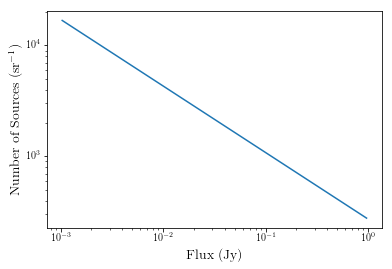
\includegraphics[width=0.6\textwidth]{dnds.png}
  \caption{Plot of Number of Sources per steradian versus Flux. Where the power law slope is equal to -0.6. }
  \label{fig:LNLS}
\end{center}
\end{figure}
When generating points at first we might think that we can randomly generate points on a 2D rectangle and then convert into sky coordinates, however because of how 2D projections of 3D objects work this causes an over density of points at the pole if converted into sky coordinates, see Figure \ref{fig:bpoint}. A better method of generating the points was found by Cory Simon\footnote{\url{corysimon.github.io/articles/uniformdistn-on-sphere/}}. As described, we can get the correct distribution of points by generating a unit cube of points and take points with a radius of 1. Points less that 1 radius are scaled up to be 1 radius away. This left us with a 3D sphere of points at unit radius away we can see this cube and sphere in Figure \ref{fig:cub+sph}
\begin{figure}[H]
    \centering
    \begin{subfigure}[t]{0.5\textwidth}
        \centering
        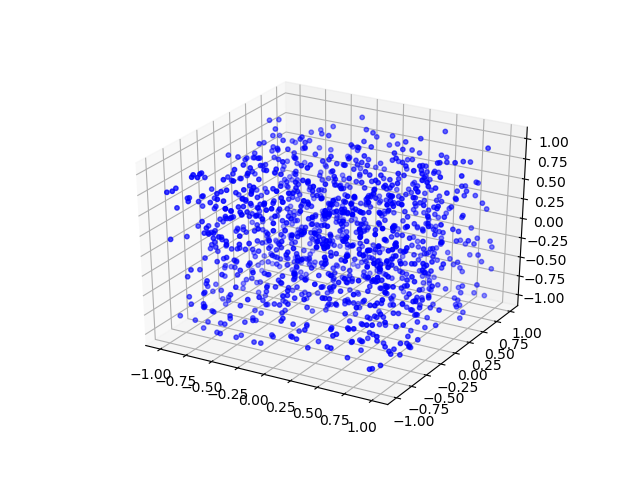
\includegraphics[width=\textwidth, right]{cube1.png}
        \caption{Cube which is -1 to 1 for all dimensions}
    \end{subfigure}%
    ~ 
    \begin{subfigure}[t]{0.5\textwidth}
        \centering
        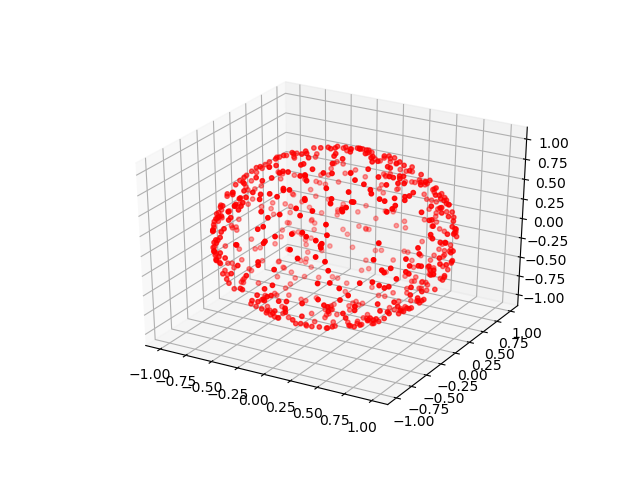
\includegraphics[width=\textwidth, left]{sphere1.png}
        \caption{Sphere of radius 1.}
    \end{subfigure}
    \caption{A comparison of unit cube generated (a) and unit sphere taken from this cube (b).}
    \label{fig:cub+sph}
\end{figure}

These points were then converted into a 2D map of the sky as seen in Figure \ref{fig:gpoint}. Once we have the distribution of points we can use the a function from \texttt{AegeanTools} \citet{Aegean} to check whether these points are within the region supplied this is done til the number of sources within the region have been generated.\\
\begin{figure}[H]
    \centering
    \begin{subfigure}[t]{0.5\textwidth}
        \centering
        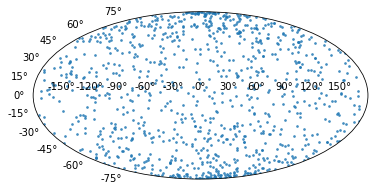
\includegraphics[width=\textwidth, right]{map_bad.png}
        \caption{Bad Point Generation}
        \label{fig:bpoint}
    \end{subfigure}%
    ~ 
    \begin{subfigure}[t]{0.5\textwidth}
        \centering
        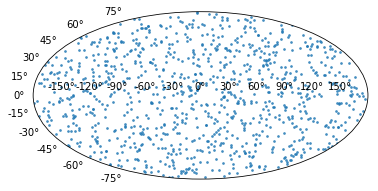
\includegraphics[width=\textwidth, left]{map_good.png}
        \caption{Good Point Generation}
        \label{fig:gpoint}
    \end{subfigure}
    \caption{A comparison between random point generation on a 2D surface converted into sky coordinates (a) and the point generation using a sphere (b).}
\end{figure}

From the previous section we know that sources can come in a wide variety but we want to categorise our sources into two types to make our simulation a little easier to do. So what we decided to do was say that there are scintillating and non-scintillating sources or compact and extended sources. Each make up a fraction of our total sources. Spectral Energy Distribution (SEDs) are intrinsically linked to the behaviour and type of source, we can use this to put limits on the different types of sources. Flat SEDs are associated with compact objects which we expect to be scintillating, whereas extended objects which do not scintillate are associated with steep SED's. Here we define flat as a SED alpha value between -0.5 to 0.5 and steep as anything lower than -0.5. To determine this fraction we used the GLEAM catalogue \citep{Gleam} and said that sources with Flat SED's were scintillating, whereas sources with steep SEDs were not scintillating \textcolor{red}{(Add Figure/Little bit more explanation about SEDs)}. This fraction turned out to be $\sim 84.84\%:15.16\%$ compact to extended.

We also made another assumption, that the source sizes of these two categories were also a constant, we determined that the source sizes of the scintillating was 2 milli-arcseconds and non-scintillating was 30 milli-arcseconds, this source size is used later when determining modulation index. \textcolor{red}{(Maybe include expanded discussion of these values)}

We now have a number of sources with their associated flux's and source type/sizes we can now use this to determine modulation using \texttt{SM2017} as discussed in Section \ref{sec:SM2017}. At this stage of the simulation \texttt{\texttt{SM2017}} has determined the modulation as well as other parameters. Now the modulation can be scaled by the refractive timescale and the observation time inputted by the user using Equation \ref{eq:modscale}.
\begin{equation}\label{eq:modscale}\mathrm{ 
m_{s}=m\bigg(\dfrac{t_{obs}}{t_{ref}}\bigg)
}\end{equation}
Where $m_s$ is the scaled modulation, $m$ is the original modulation index calculated by \texttt{\texttt{SM2017}}. $t_{obs}$ is the observation time inputted by the user. and $t_{ref}$ is the refractive timescale calculated by \texttt{\texttt{SM2017}}.
 
We then want to count number of sources above some modulation index, we used m=0.05 (5\%) as seen in (\textcolor{red}{ref Hancock/Bell(?)}) and counted how many sources were above this limit, however this is a changeable parameter. We then divide the number of modular sources by the area to get the number of variable sources per square degree (Equation \ref{ASD}, also known as the Areal Sky Density (ASD). We can then run this multiple times to get statistics about the ASD.\\
\begin{equation}\mathrm{\label{ASD}
    ASD=\dfrac{N_{var}}{Area}
}\end{equation}

The program returns two files (if the option is selected) the first is the `data' file which contains the average and standard deviation of all the important parameters (Ha, t0, theta, mod)  for each iteration. The second file is the 'results' file which shows the average of all those important parameters over the entire number of iterations. It also shows the input conditions which have been used.\\
\begin{figure}[H]
    \centering
    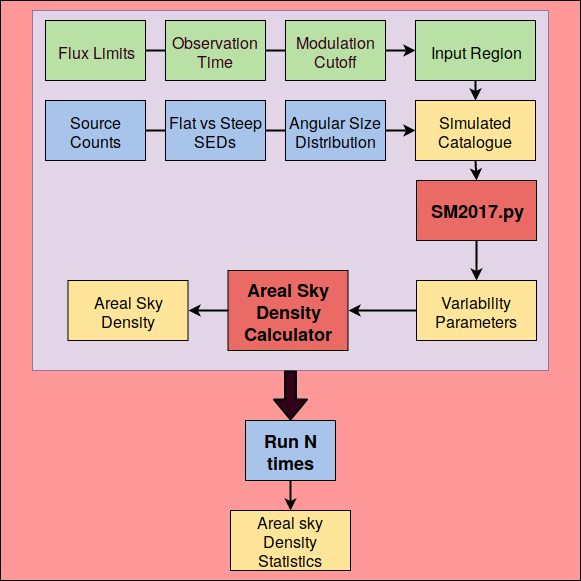
\includegraphics[width=0.6\textwidth]{SIM3(1).png}
    \caption{The SIM.py program flowchat, where Green are the inputs from the user, blue are the simulation variables, yellow are the results, and Red represent Programs and functions.}
    \label{fig:SIM}
\end{figure}

Figure \ref{fig:SIM} shows a flowchart of the \texttt{SIM.py} program including the main inputs and simulation parameters used. The program can take in multiple parameters from the user and has defaults assigned to each show in brackets: Lower flux limit (1 mJy), upper flux limit (1 Jy), modulation cutoff (0.05), observation time (183 days), alpha scaling constant (3300), frequency (185 MHz), number of iterations (20), region file name and output file name. Most of these have default values but the region file name is required, the program will output key details to the user terminal unless output file name is specified.


\subsection{Limitations}
In the programs current state it runs quite well but is a little slow on larger amounts of iterations, this could probably be fixed by improving some of the clunkier code that the simulation runs on. I think there are certain parts of the program that could be streamlined with enough time such as the source generation. The source generation over estimates the number of points and then cuts them down to the right amount. This takes longer to generate and is one of the many areas where the code could be improved.\\

The source size is still fairly basic and makes a good estimate towards characteristic size of sources that will and wont scintillate. However I think this could be improved upon by having a source size distribution function either based on flux, frequency, position or maybe a combination of those.\\

The distribution of flat/steep SEDs is generated across the whole GLEAM catalogue and isn't specific to the flux regime that the survey might be in. This could be improved quite easily by just including a function to generate the flat to steep ratio for each flux bin that is created during the source count function within the simulation. \textcolor{red}{As suggested by Ben Quici} we could also use cross matched catalogues with GLEAM that are of higher resolution (TGSS) to see if sources are consistently flat/steep. From this we can work out the number of "steep" sources that are flat and the number of "flat" sources that are steep.\\


\section{Results and Discussion}
 This project work is being done alongside processing for the MWA Project G0003 lead by Dr. Paul Hancock. We will be using the survey regions from this project to compare our results and see if they are in agreement. This project is herein referenced as the High Galactic Latitude (HGL) survey. The HGL survey  was done at 185 MHz with several different regions, HGL5, HGL6, HGL7 and HGL8, Table \ref{tab:regs} shows the positions of each of these surveys, each region had an area of 628 square degrees.\\


\begin{table}[H]
\centering
\begin{tabular}{cccccc}
\toprule
\textbf{Region} &\textbf{l (deg)}   & \textbf{b (deg)}    & \textbf{Radius (deg)}\\\midrule

\textbf{HGL 5}  & 198 & -79.5 & 15 \\
\textbf{HGL 6}  & 209 & -55.3 & 15 \\
\textbf{HGL 7}  & 208 & -39.4& 15 \\
\textbf{HGL 8}  & 205 & -16.3 & 15 \\\bottomrule
\end{tabular}
\caption{Coordinates of all regions from the HGL survey in galactic coordinates measured in degrees and J200 coordinates.}
\label{tab:regs}
\end{table}

%I am also going to compare my work to a higher frequency survey, the Phoenix Deep Survey (PDS). Hancock et al (REF) compare several different surveys within this paper, which allows me to compare my results from the HGL simulations and several other simulations at higher frequency using the PDS regions.\\
\subsection{Output}
Running the simulation for each of the HGL regions using the input parameters of a flux density limit of 60 mJy, an assumed flux upper limit of 1 Jy, observation time of 365 days, a scaling factor (a) of 3300, and a modulation cut off of 0.05 was also assumed. The output from the program is received as two files, one the full data from each iteration (data file) and one of the averaged results and input parameter (results file). 
\begin{figure}[H]
\begin{center}
  \includegraphics[scale=0.8]{ASD_hist7f.png}
  \caption{Histograms of the Areal Sky Density for HGL 7, run for 100 iterations at 185 MHz (Blue) and 1400 MHz (Red). For each frequency the mean and standard deviation are shown in the respective colours.}
  \label{fig:ADS1}
\end{center}
\end{figure}
In Figure \ref{fig:ADS1} we can see and example of the ASD results from the simulation for the HGL 7 region run for 100 iterations at 185 MHz and 1400 MHz. We can compare this result to other surveys, using a figure from Hancock et al, Figure \ref{fig:comp}

\begin{figure}[H]
\begin{center}
  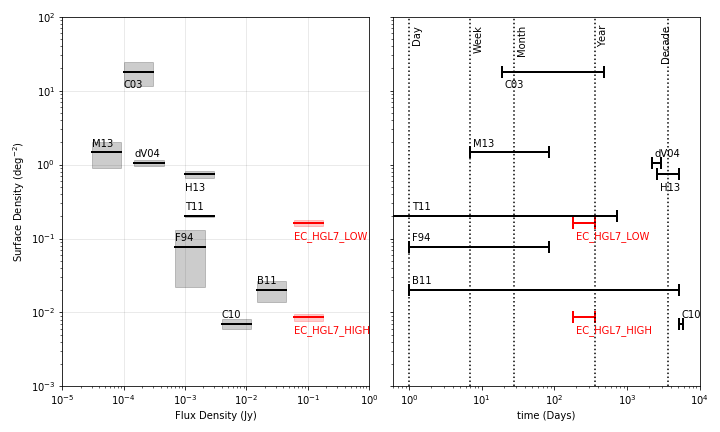
\includegraphics[width=\textwidth]{lognlogs2.png}
  \caption{Figure adapted from \citet{PDS_PJH} comparing surface density against flux density (left) and timescale (right) of different surveys. Included are the results from our simulation where blue is the 185 MHz simulation and red is the 1400 MHz simulation.  References are: C03 - \citet{Carilli03}, M13 - \citet{Mooley13}, dV04 - \citet{deVires04}, H13 - \citet{Hodge13}, F94 - \citet{Frail94}, C10 - \citet{Croft10}, B11 - \citet{Bannister11}, T11 - \citet{Thyag11}, PH16 - \citet{PDS_PJH}}
  \label{fig:comp}
\end{center}
\end{figure}
In Figure \ref{fig:comp} all of the other lines represent other surveys all taken from 800 MHz to 1400 MHz, much higher frequency than the HGL survey. But our 1400 MHz simulation agrees with the other results! This is great because it shows that our simulation produces results that are in agreement with several other surveys. However it is harder to compare our 185 MHz results as previously mentioned these surveys are at much higher frequencies. Instead we can directly compare results obtained from our simulation with results obtained directly from Dr Paul Hancock's analysis of the HGL regions.\\

A comparison of these values for HGL regions 7 and 8 can be seen in Table \ref{tab:HGLcomp}. SIM 7 has very good agreement with the HGL 7 results which shows that the simulation can return results. However SIM 6 and SIM 8 both do not agree with the HGL results. 
\begin{table}[H]
    \centering
\begin{tabular}{llll}
    \toprule
    \textbf{Region}	& \textbf{Sources}	&	\textbf{Variables}	&		\textbf{ASD}		\\ \midrule
    \textbf{HGL 6}	&   5391 &	16 $\pm$ 4  &	0.022 $\pm$ 0.006	\\
    \textbf{SIM 6}	&	5259 &  425 $\pm$ 21&	0.59  $\pm$ 0.03	\\\midrule
    \textbf{HGL 7}	&	4678 &	14 $\pm$ 4	&	0.022 $\pm$ 0.006	\\
    \textbf{SIM 7}	&	4587 &	11 $\pm$ 3	&	0.017 $\pm$ 0.005	\\\midrule
    \textbf{HGL 8}	&	3672 &	8 $\pm$ 3 	&	0.013 $\pm$ 0.005	\\
    \textbf{SIM 8}	&   3606 &	1 $\pm$ 1	&	0.0005 $\pm$ 0.0005	\\\bottomrule
\end{tabular}
    \caption{Table comparing the actual results variability results from HGL regions to the simulated results. Errors have been calculated using Poisson statistics.}
    \label{tab:HGLcomp}
\end{table}

After investigating what could be causing the discrepancy it was found that the \halpha values for the HGL 6 region were dominated by noise with the \halpha error being on order of 10-30 times greater than the actual \halpha value. This noise dominated region is occurring at the poles of the \halpha maps where they have low resolution data and incomplete regions leading to this large error dominating any actual scattering that could occur. So it is most likely that the discrepancy in SIM 6 is due to the position of HGL 6 being in a very noisy region of the \halpha input maps. I was unable to correct this error in time however with the noise being approximately 10-30 times greater we can assume that our SIM 6 region could be producing results that are at a maximum  an order of 30 out from the correct answer, which is what we see in Table \ref{tab:HGLcomp}.\\

\begin{figure}[H]
\begin{center}
  %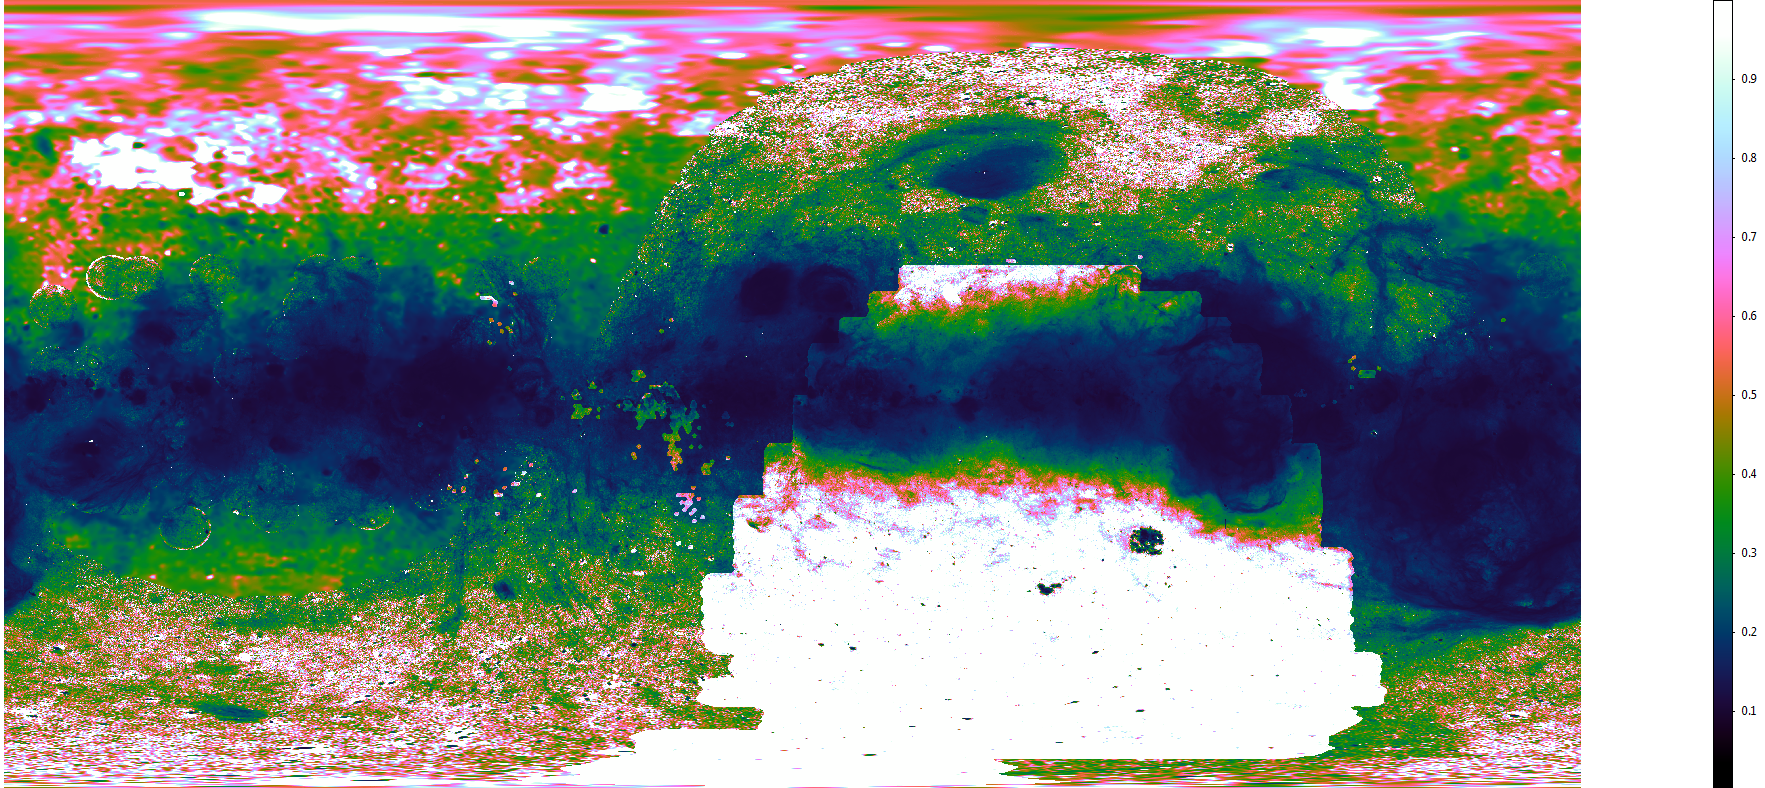
\includegraphics[width=\textwidth]{HA_err.png}
  \caption{Image showing the relative error map ($\Delta$\halpha/ \halpha) colour bar shows the darkest colour (black) as the lowest relative error and brightest colour (white) as the largest relative error.}
  \label{fig:comp}
\end{center}
\end{figure}
However this issue could not be causing the discrepancy in SIM 8 as the HGL 8 region lies closer to the galactic plane (Table \ref{tab:regs}). I decided to look at where this region was in the sky and to see if there was anything unusual that might be causing a disagreement. It turns out that this region was encompassing the Orion nebula, this is an issue because the Orion nebula is 412 parsec's away and as mentioned in Section \ref{sec:SM2017} the \sm program makes the basic assumption that the scattering screen is a distance of 1 kpc away.
\begin{wrapfigure}{r}{0.41\textwidth}
  \vspace{-20pt}
  \begin{center}
    %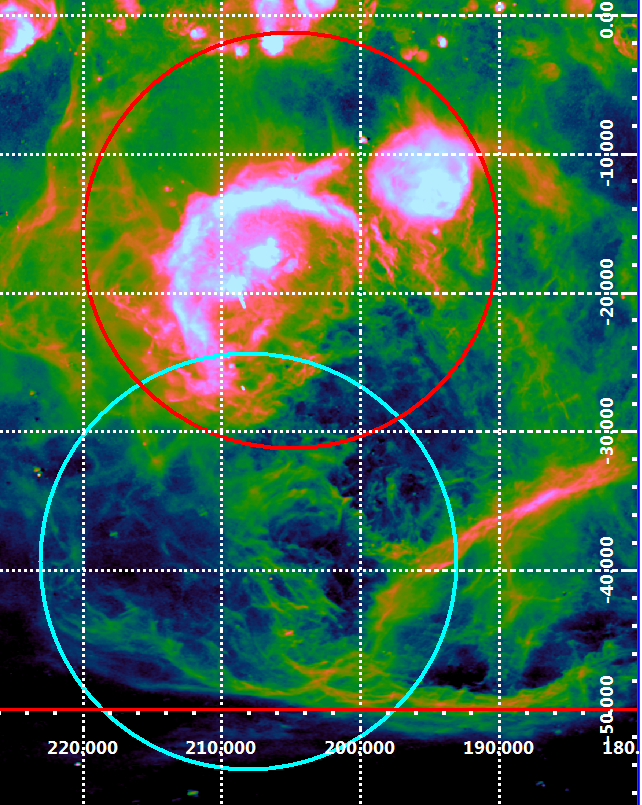
\includegraphics[width=0.4\textwidth]{HG78_grid.PNG}
  \end{center}
  \vspace{-20pt}
  \caption{Image showing regions HGL 8 (red), HGL 7 (teal), overlayed on the Hydrogen Alpha map.}
  \label{fig:HAreg}
  \vspace{-10pt}
\end{wrapfigure}
This means that our scattering screen is behind where the majority of this \halpha is coming from and thus is not accounting for any of the scattering that should occur. Changing the scattering screen distance to be 412 pc in the \texttt{SM2017} program we get a result of 40 $\pm$ 6 variable sources and a ASD of 0.064 $\pm$ 0.01, which is in much better agreement with our results. In Figure \ref{fig:HAreg} we can see how HGL 8 (red) is positioned on top of the bright Orion Nebula which causes this disagreement due to distance assumptions, where as the HGL 7 (teal) region is not over the Orion nebula and over some general \halpha region from the galactic plane where the distance model is more accurate.

From the above it is found that it is not the Simulation that is causing disagreements but rather some underlying assumptions and models within \sm, specifically the \halpha maps high noise regions causing over densities of variables sources. This could be resolved by obtaining updated \halpha maps that have higher resolution and have no missing regions. The other issue being the simple distance model causing under densities in regions where the majority of the \halpha is closer to us than the actual screen. This could also be resolved using more complex distance models such as a pancake distance model which is better, but still not great as it ignores local features such as the Orion nebula. However I think this is being worked on by Dr Paul Hancock in his evolution of the SM2017 model.
\textcolor{red}{Emphasise SM2017 being the issue more? or is that enough? include corrected table? (see below)}
\begin{table}[H]
    \centering
\begin{tabular}{llll}
    \toprule
    \textbf{Region}	& \textbf{Sources}	&	\textbf{Variables}	&		\textbf{ASD}		\\ \midrule

    \textbf{HGL 7}	&	4678 &	14 $\pm$ 4	&	0.022 $\pm$ 0.006	\\
    \textbf{SIM 7}	&	4587 &	11 $\pm$ 3	&	0.017 $\pm$ 0.005	\\\midrule
    \textbf{HGL 8}	&	3672 &	8 $\pm$ 3 	&	0.013 $\pm$ 0.005	\\
    \textbf{SIM 8}	&   3606 &	40 $\pm$ 6	&	0.06 $\pm$ 0.01	\\\bottomrule
\end{tabular}
    \caption{Corrected HGL 8 results.}
    \label{tab:HGLcorr}
\end{table}
\subsection{Comparison to HGL/Pauls results}
% Area = 627.73 deg^2

\textcolor{red}{Ignore below table, just keeping values for reference atm}
\begin{table}[H]
    \centering
\begin{tabular}{lllll}
    \toprule
    \textbf{Region}	&	\textbf{Variables}	&	\textbf{Sources}	&	\textbf{ASD}	&	\textbf{Error \%}	\\ \midrule
    \textbf{HGL\_5}	&	9	&	4505	&	0.0143	&	0.00	\\
    \textbf{SIM\_5}	&	689	&	4586	&	1.098	&	98.70	\\
    \textbf{SIM\_5(183)}	&	424	&	4586	&	0.675	&	97.88	\\\midrule
    									
    \textbf{HGL\_6}	&	16	&	5391	&	0.0223	&	0.00	\\
    \textbf{SIM\_6}	&	425	&	5259	&	0.5916	&	96.23	\\
    \textbf{SIM\_6(183)}	&	107	&	5259	&	0.0151	&	47.68	\\\midrule
    									
    \textbf{HGL\_7}	&	14	&	4678	&	0.0222	&	0.00	\\
    \textbf{SIM\_7}	&	11	&	4587	&	0.0174	&	36.20	\\
    \textbf{SIM\_7(183})	&	0.67	&	4587	&	0.0011	&	1,918.18	\\\midrule
    \textbf{HGL\_8}	&	8	&	3672	&	0.01274	&	0.00	\\
    \textbf{SIM\_8}	&	0.89	&	3606	&	0.000498	&	2,458.23	\\
    \textbf{SIM\_8(183)}	&	0.93	&	3606	&	0.00148	&	760.81	\\\bottomrule
\end{tabular}
    \label{tab:Hp}
    \caption{185 MHz, 100 iterations, 365 days, 60mJy LFD, 3300a for all except 2600a for HGL8}
\end{table}
%Looking at Table \ref{tab:HGL_comp} we can see the results from the HGL survey as well as the simulated results by our program at two different time scales, 365 days and 183 days. At the 365 day timescale the results for Region 7 are very good being with a 36.2\% error, Regions 5 and 6 also agree fairly well, both being within a 100\% error margin. Region 8 has the most disagreement and this is likely due to ?????????????. Speculation: Either increased H alpha value or distance need to print distance out to check this.

\subsection{Comparison to PDS survey}
\textcolor{red}{PDS area results kept returning 0 variability think area is either too small or maybe its another latitude thing, will try work out. (Later found) This is in the noise dominated region of the map so results are pretty crap here probably why it couldnt find anything.}
\subsection{How much the results agree}
\subsection{What may have caused differences}

\subsection{What can be improved}
\begin{itemize}
    \item Distance Model
    \item Better \halpha maps
    \item SED dist per flux bin
    \item Source Distribution (Spacial clustering/two point correlation)
\end{itemize}
\section{Conclusion}
\subsection{Summary of results}
\subsection{Summary of discussion}
\subsection{What was found and what can be done in the future.}




%\bibliography{export-bibtex.bbl} % if your bibtex file is called example.bib

\bibliographystyle{abbrvnat}
% Alternatively you could enter them by hand, like this:
% This method is tedious and prone to error if you have lots of references
\begin{thebibliography}{99}
\bibitem[\protect\citeauthoryear{Camenzind}{2007}]{2007coaw.book.....C} Camenzind M., 2007, coaw.book.
\bibitem[\protect\citeauthoryear{Cordes \& Lazio}{2002}]{2002astro.ph..7156C} Cordes J.~M., Lazio T.~J.~W., 2002, astro, arXiv:astro-ph/0207156 
\bibitem[\protect\citeauthoryear{Cordes \& Lazio}{2003}]{2003astro.ph..1598C} Cordes J.~M., Lazio T.~J.~W., 2003, astro, arXiv:astro-ph/0301598 
\bibitem[\protect\citeauthoryear{Dubner \& Giacani}{2015}]{2015A&ARv..23....3D} Dubner G., Giacani E., 2015, A\&ARv, 23, 3 
\bibitem[\protect\citeauthoryear{Ginzburg \& Syrovatskii}{1965}]{1965ARA&A...3..297G} Ginzburg V.~L., Syrovatskii S.~I., 1965, ARA\&A, 3, 297 
\bibitem[\protect\citeauthoryear{Lorimer \& Kramer}{2012}]{2012hpa..book.....L} Lorimer D.~R., Kramer M., 2012, hpa..book,
\bibitem[\protect\citeauthoryear{Macquart \& Koay}{2013}]{JP} Macquart J.-P., Koay J.~Y., 2013, ApJ, 776, 125 
\bibitem[\protect\citeauthoryear{Mayer, McCullough, \& Sloanaker}{1957}]{1957ApJ...126..468M} Mayer C.~H., McCullough T.~P., Sloanaker R.~M., 1957, ApJ, 126, 468 
\bibitem[\protect\citeauthoryear{Narayan}{1992}]{Narayan} Narayan R., 1992, RSPTA, 341, 151 
\bibitem[\protect\citeauthoryear{Scheuer}{1968}]{1968Natur.218..920S} Scheuer P.~A.~G., 1968, Natur, 218, 920 
\bibitem[\protect\citeauthoryear{Walker}{1998}]{Walker} Walker M.~A., 1998, MNRAS, 294, 307 
\bibitem[\protect\citeauthoryear{Hancock et al.}{2016}]{PDS_PJH} Hancock P.~J., Drury J.~A., Bell M.~E., Murphy T., Gaensler B.~M., 2016, MNRAS, 461, 3314 
\bibitem[\protect\citeauthoryear{Haffner, Reynolds, \& Tufte}{1998}]{Haffner} Haffner L.~M., Reynolds R.~J., Tufte S.~L., 1998, ApJ, 501, L83 
\bibitem[\protect\citeauthoryear{Hurley-Walker et al.}{2017}]{Gleam} Hurley-Walker N., et al., 2017, MNRAS, 464, 1146 
\bibitem[\protect\citeauthoryear{Armstrong, Rickett, \& Spangler}{1995}]{Armstrong} Armstrong J.~W., Rickett B.~J., Spangler S.~R., 1995, ApJ, 443, 209 
\bibitem[\protect\citeauthoryear{Hancock et al.}{2012}]{Aegean} Hancock P.~J., Murphy T., Gaensler B.~M., Hopkins A., Curran J.~R., 2012, MNRAS, 422, 1812 
\bibitem[\protect\citeauthoryear{Intema et al.}{2011}]{Intema} Intema H.~T., van Weeren R.~J., R{\"o}ttgering H.~J.~A., Lal D.~V., 2011, A\&A, 535, A38 
\end{thebibliography}


%\textbf{Harcastle M. 2006.} Radio galaxy 3C98 \& 3C31. %\url{https://en.wikipedia.org/wiki/File:Radio_galaxy_3C98.png}.\\
%\textbf{Jansky K.G. 1932.} Directional Studies of Atmospherics at High Frequencies. In: Classics in Radio Astronomy. Studies in the History of Modern Science, vol 10. Springer, Dordrecht. doi:https://doi.org/10.1007/978-94-009-7752-5\_1.\\
%\textbf{Kembavi \& Narlikar. 1999.} 9.3 FANAROFF-RILEY CLASSIFICATION.
%\url{https://ned.ipac.caltech.edu/level5/Glossary/Essay_fanaroff.html}.\\
\bsp	% typesetting comment
\label{lastpage}
\end{document}
